\begin{frame}
\frametitle{The neutron becomes the neutrino}
\begin{columns}
\column{0.35\textwidth}
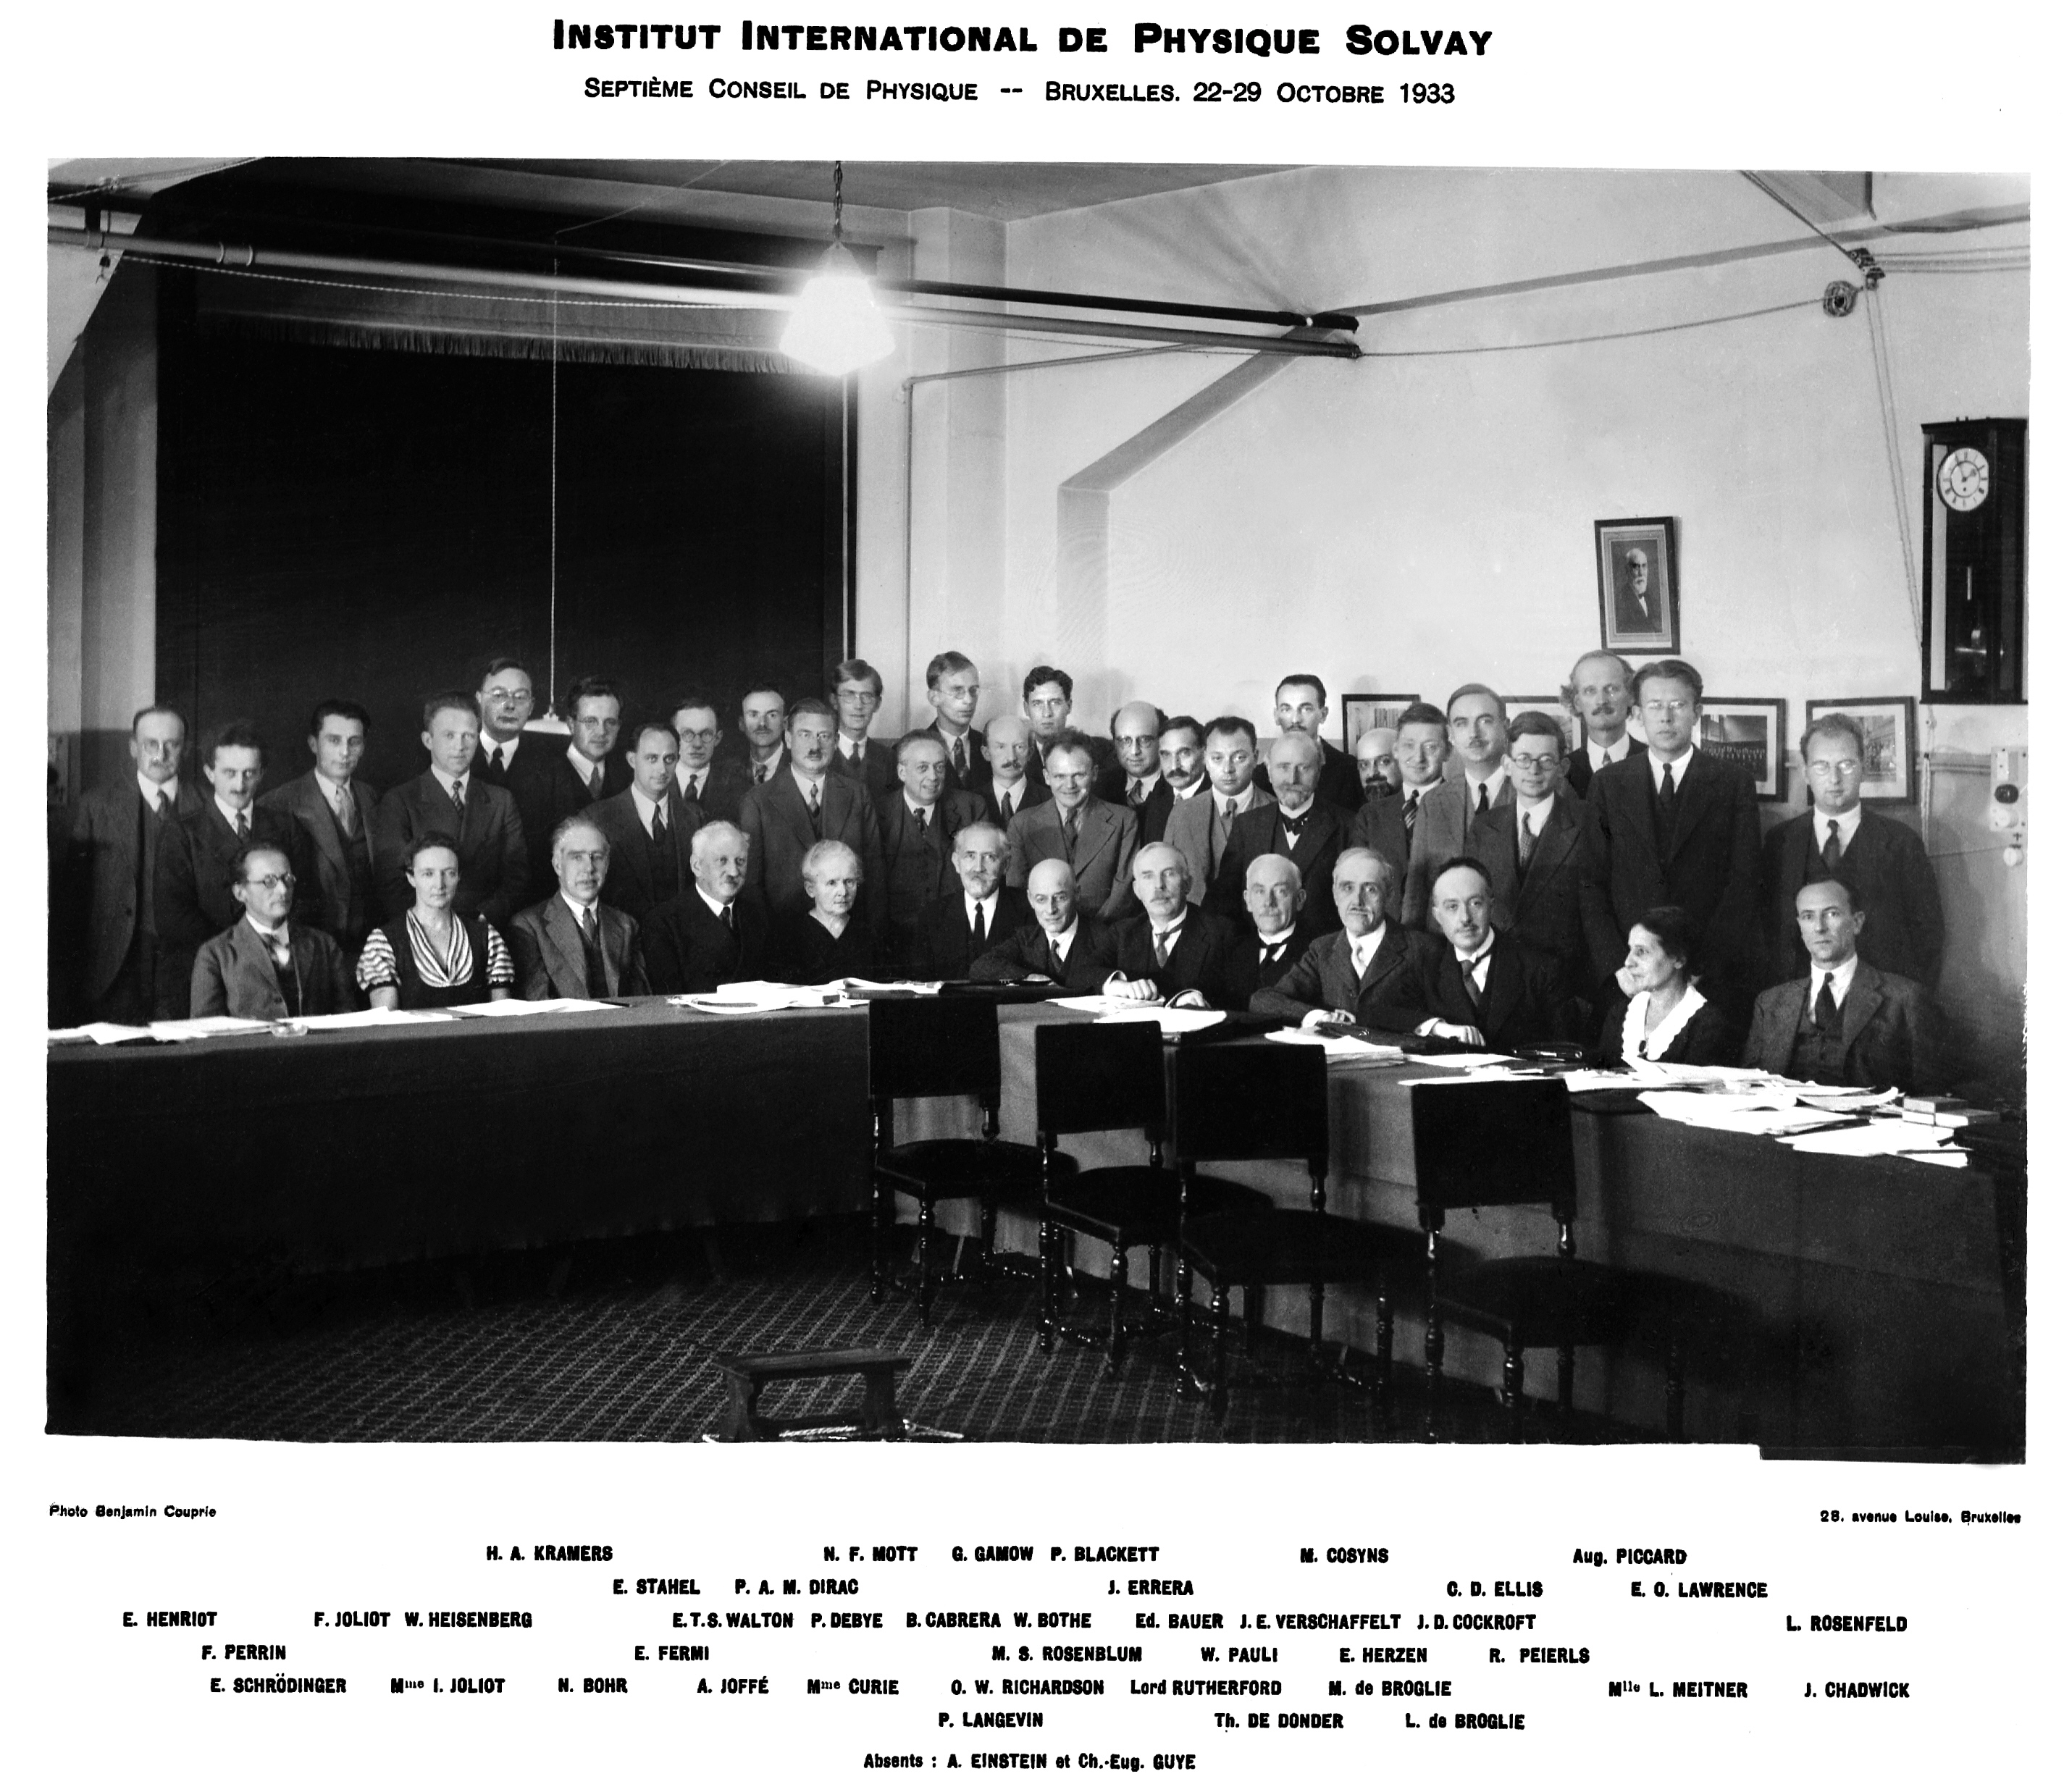
\includegraphics[scale=0.18]{Solvay1933Large.jpg}
 
 \column{0.6\textwidth}
%\begin{block}{}
Pauli in  1933 at the Solvay Congress: ``Regarding the properties of these neutral particles, the atomic weights
of the radioactive elements tell us first of all that their mass cannot exceed
much that of the electron. In order to distinguish them from the heavy
neutrons, Mr. Fermi proposed the name ``neutrino.'' {\bf It's possible that the
neutrinos' own mass might be equal to zero, so that they would have to
propagate with the speed of light, like the photons}. However, their penetrating power would exceed by far that of photons of the same energy. It
seems to me acceptable that the neutrinos have spin 1/2 and satisfy Fermi's 
statistics, although experiments do not give us any direct proof of this hypothesis. 
{\bf We know nothing about the interaction of the neutrinos with other material particles and with the photons".}

%\end{block}
\end{columns}
\end{frame}
